%\section{Background}
\label{sec:bpm2015background}

Business process management plays an important role for improving the performance and compliance of various types of processes. In practice, many processes are executed with clear guidelines and regulatory rules, but without an explicit centralized control imposed by a process engine. In particular, it is often important to exactly know when which work was done. This is, for instance, the case for complex engineering processes in which different parties are involved. We refer to this class of processes as project-oriented business processes.

Such project-oriented business processes are difficult to control due to the lack of a centralized process engine. However, there are various unstructured pieces of information available to analyze and monitor their progress. One type of data that are often available these processes is event data from version control systems (VCS). While process mining techniques provide a useful perspective on how such event data can be analyzed, they do not produce output that is readily organized according to the project orientation of these processes.

In this thesis, we define formal concepts for capturing project-oriented processes. These concepts provide the foundation for us to develop an automatic discovery technique which we refer to as \emph{project mining}. The output of our project mining algorithm is organized according to the specific structure typically encountered in project-oriented business processes. With this work, we extend the field of process mining towards the coverage of this specific type of business process.


Next, we describe the addressed problem and related work.


\subsection{Problem Description}\label{sec:bpm2015problem}
The class of processes that we discuss in this paper are long-term engineering projects. These processes have specific requirements for monitoring. First, they are executed only once according to the specific needs of a particular project, and only partially according to recurring process descriptions. Second, they involve various actors that typically document their work in a semi-structured way using text and tables. Third, work in the project is usually subject to constraints regarding the start and end and the temporal order. Fourth, there is typically no process engine controlling the execution. Fifth, even though these limitations in terms of traceability exist, there are usually strong requirements in terms of tracking when which work was conducted.

%Unlike other types of business processes, the processes we consider here
%representing such projects are specifically tailored to customer needs the specific needs of the project, and there is

In line with these observations, a \textit{project-oriented business process} can be defined as an ad-hoc plan that specifies the tasks to be performed within a limited period of time and with a limited set of resources for achieving a specific goal. Unlike repetitive business processes for which notations such as BPMN~\citep{bpmn2_stable} or EPC~\citep{vanderaalst_formalization_1999} are commonly used, project-oriented business processes may be properly represented with PERT or GANTT models. The concept is illustrated in Fig.~\ref{fig:bpm2015problem}.


\begin{figure}[tb]
\centering
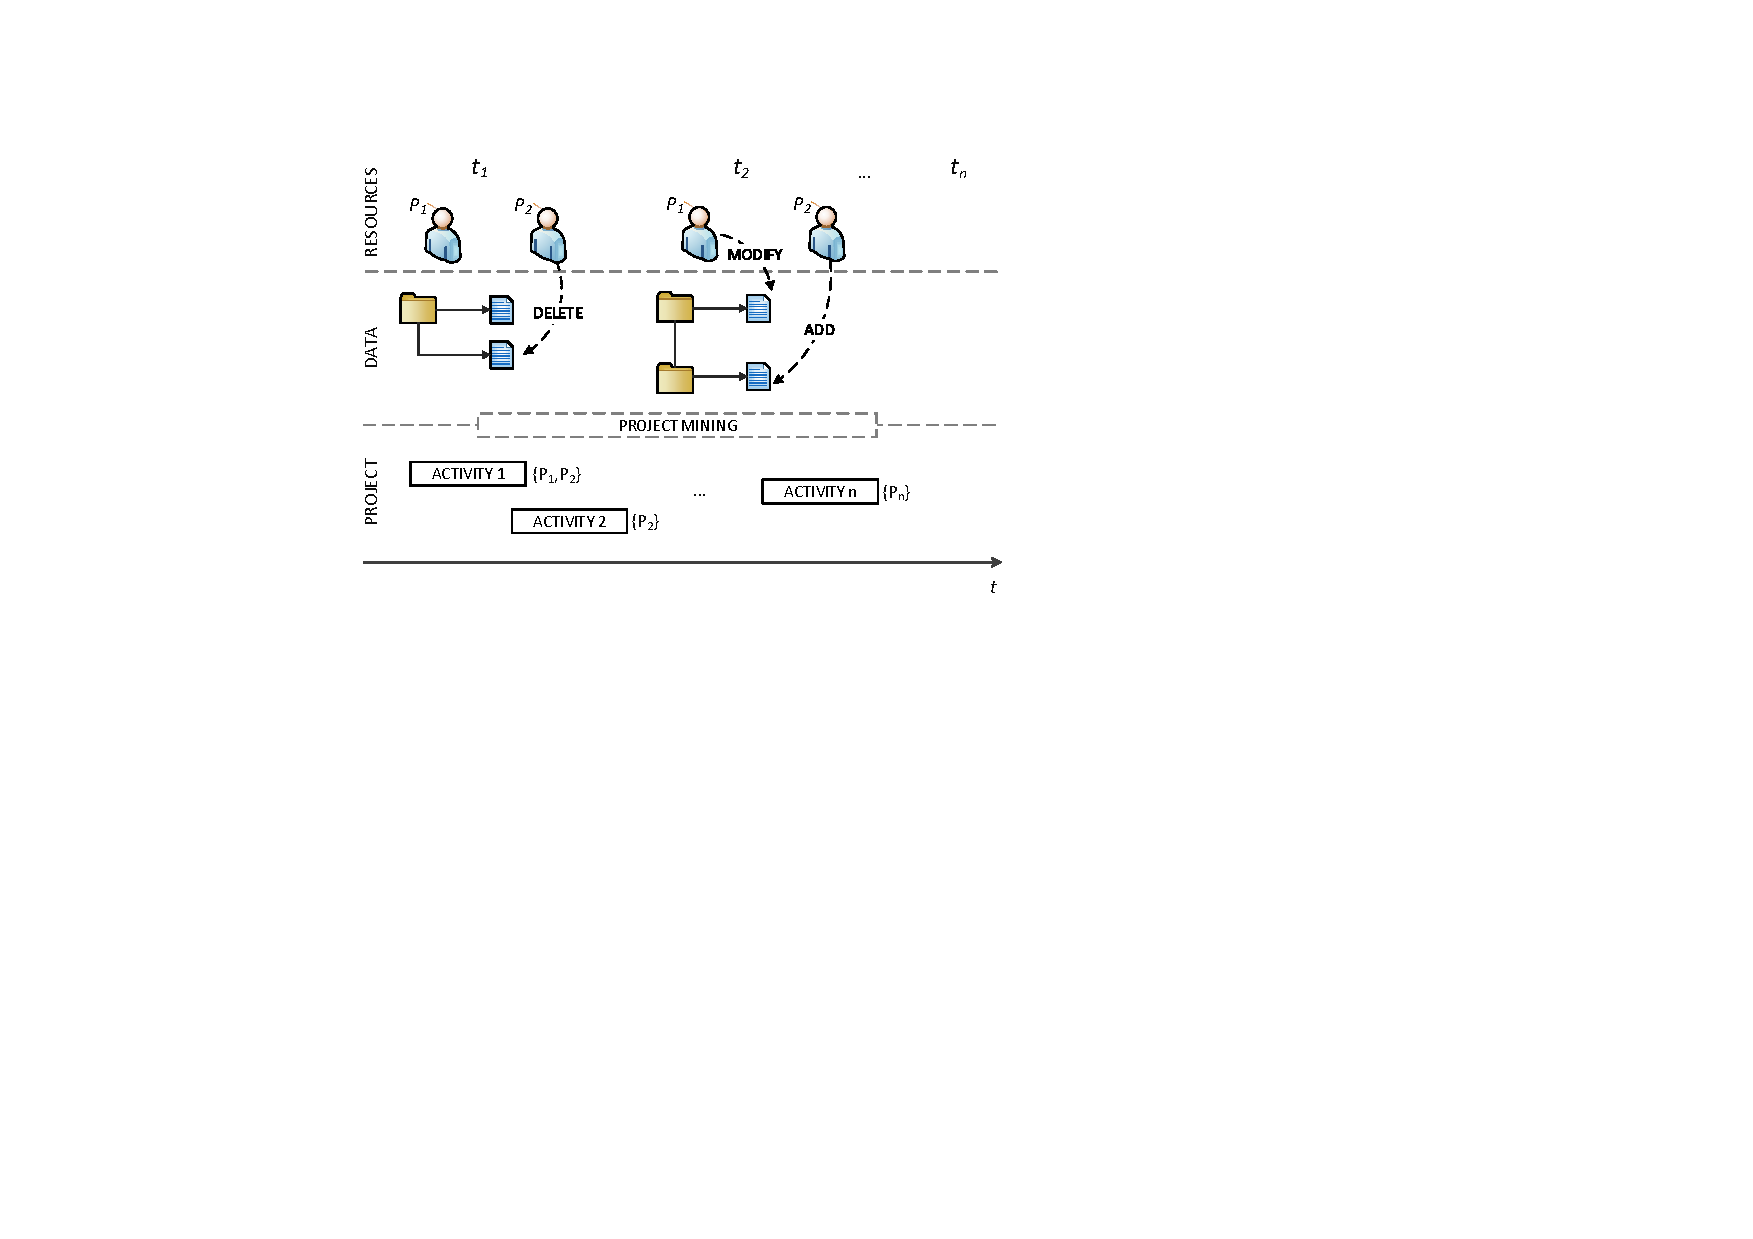
\includegraphics[width=.8\textwidth]{bpm2015/imgs/ProjectMining.pdf}
\caption{Gap between User-Generated Artifacts and Project-Activities}
\label{fig:bpm2015problem}
\end{figure}

Documentation is required not only explicitly as part of some activities but also to comply with norms and regulations that may require some evidence of the actions being performed in the organization. Documents are usually free of format or contain tables, at best. The unstructuredness of data makes it difficult to monitor processes and check rules on them. A starting point for analysis of project-oriented processes can be data logs %generated for  %usually consist of subversion projects
that are stored in Software Configuration Management (SCM) systems that help tracking the evolution of data and restore information if needed~\citep{voinea_open_2006}.
However, hundreds of versions of thousands of files are common in a single project~\citep{voinea_multiscale_2006}, which makes it impractical to browse this data manually.

%We focus on project mining motivated by a real case scenario in the scope of the SHAPE research project\footnote{\url{http://ai.wu.ac.at/shape-project/}}.
%The data log is provided by a Version Control Systems (VCS) whose information is not subdivided into traces related to process instances but consists of a hierarchy of work streams associated with individual files being added, modified or deleted in a subversion repository.

Let us see an example inspired by a real scenario of a process to write a project proposal that uses a Version Control System (VCS) to store the data. The project history, and hence, the data produced, starts when people begin to work on the proposal, which involves a description of the project goals and milestones, a division of tasks into work packages, an estimation of cost and resources required, etcetera. This information is spread in the repository over several folders containing different documents, which are later merged into a single file. If the proposal is accepted, the first step is to organize a kickoff meeting and assign specific resources to the work packages. A hierarchical set of folders is then created in the repository in order to store the information generated for each work package. As the project evolves over time, resources contribute by adding, removing or modifying information to the VCS repository. %\todo{Should answer point 3 on the review-list: Missing concrete examples of the need to “prove compliance to rules and regulations”. Which important rules and regulations will the analysis help comply with?} 
Project evolution is guided by specific norms that impose the execution of predefined steps. For instance, the European norm EN5016 requires a preliminary \gls{ram} analysis to support targets. 
%Data stored in the VCS can be used to prove compliance to rules and regulations of the domain. For instance, in the railway industry, 

Table~\ref{tab:bpm2015example} depicts an excerpt of the log data generated, where the first column (on the left hand side) indicates the commit identifier, the second column indicates the person who committed changes, the third column indicates the commit date, %the fourth column shows (optional) descriptive information to clarify the scope of the changes performed
and the fourth column indicates the files affected and the type of action performed among added (A), modified (M) and deleted (D).
For the sake of simplicity, the table shows the log data of a specific time period and the actions related to a specific task, namely, $\defineExample$. That task was assigned to resource X % after a project meeting. %, when a part of project members asked for a toy example to better understand the problem domain.
and was supervised by resource Y and, later on, also by resource Z.
%An extract from the log concerning this period, that shows some crucial steps in the \emph{example} task, is reported on table \ref{tab:example}. Comments were left out from this representation, since at the current state we don't delve into them.

\begin{table}[bt]
\caption{Excerpt from VCS log data for the referenced time period }
\label{tab:bpm2015example}
%\scriptsize
{
%	\renewcommand{\arraystretch}{1.3}
\centering
%\fontfamily{phv}\fontseries{mc}\selectfont
\begin{tabular}{m{.8cm} m{1.5cm} m{3cm} p{5.8cm}}
%\hline\noalign{\smallskip}
%\hline
\toprule
\textbf{CID}	 & \textbf{Resource} & \textbf{Date} & \textbf{List of changes} \\
%\noalign{\smallskip}
%\hline
%\noalign{\smallskip}
%\hline
\midrule
%\noalign{\smallskip}
\multirow{2}{*}{1} & \multirow{2}{*}{Y} & \multirow{2}{*}{2014-11-12~11:57:46} & A /example \\
& & & A \slash example\slash SHAPE\slash\-ToyStation\-Example.docx \\ \midrule %\hdashline

%\multirow{2}{*}{205} & \multirow{2}{*}{X} & \multirow{2}{*}{2014-11-14 16:26:23} & A /example/ToyStation.bpmn \\
%& & & A /example/ToyStation.png \\ \hline %\hdashline

\ldots & \ldots & \ldots & \ldots \\ \midrule

%\noalign{\smallskip}
\multirow{2}{*}{3} & \multirow{2}{*}{X} & \multirow{2}{*}{2014-11-14 16:34:07} & M /example/ToyStation.bpmn\\
& & & M /example/ToyStation.png \\ \midrule%\hdashline

%\multirow{7}{*}{207} & \multirow{7}{*}{X} & \multirow{7}{*}{2014-11-27 14:18:59} & M /example/SHAPE-ToyStation-Example.docx \\
%& & & D /example/ToyStation.bpmn \\
%& & & M /example/ToyStation.png \\
%& & & A /example/ToyStation\_0Loop.bpmn \\
%& & & A /example/ToyStation\_1Loop.bpmn \\
%& & & A /example/ToyStation\_nLoop.bpmn \\
%& & & A/example/ToyStation\_old.bpmn\\ \hline

%\ldots & \ldots & \ldots & \ldots \\ \hline

%\noalign{\smallskip}
4 & W & 2014-12-15 13:49:11 & D /example/Download \\ \midrule %\hdashline

%\noalign{\smallskip}
5 & W & 2015-01-08 16:06:41 & A /example/Download2\\ \midrule %\hdashline

%\noalign{\smallskip}
\multirow{2}{*}{6} & \multirow{2}{*}{X} & \multirow{2}{*}{2015-01-13 11:47:09} & M /example/ToyStation\_0Loop.bpmn\\
& & & M /example/ToyStation\_nLoop.bpmn \\ \midrule %\hdashline

%\noalign{\smallskip}
\multirow{2}{*}{7} & \multirow{2}{*}{Z} & \multirow{2}{*}{2015-01-16 16:50:29} & A /example/ToyStation\_0Loop.pdf\\
& & & A /example/ToyStation-feedbackZ.pdf\\ \bottomrule %\hdashline
\end{tabular}\\ 
}
\end{table}

%Process mining techniques can help to discover processes from log data.
%Existing process mining techniques can deal very well with execution logs whose data is subdivided into \textit{traces} representing different process instances in which events are easily identifiable (e.g. through a \textit{caseId}).
%Procedural (e.g. BPMN~\citep{bpmn2_stable}, Petri nets~\citep{aalst_application_1998}, EPC~\citep{vanderaalst_formalization_1999}) as well as declarative (e.g. Declare~\citep{VanderAalst2009}, DPIL~\citep{zeising2014towards}) modeling languages can be used to represent the process discovered.
%Once a process model is discovered, it can be checked whether it is compliant with the existing (already known) process model and enhance the model or the way the process is executed accordingly.
%Performance can also be analyzed and compared to the expected values defined by key performance indicators (KPIs)~\citep{delrioortega_definition_2013}.

%\begin{table}[bt]
%\caption{Process mining vs. project mining}\label{tab:processVSprojectmining}
%\centering
%\begin{tabular}{l c c}
%%\hline\noalign{\smallskip}
%%\hline
% ~&~  Process Mining~&~Project Mining\\
%%\noalign{\smallskip}
%\hline
%%\noalign{\smallskip}
%Defined goals~&~  \cmark ~&~ \cmark \\
%Resource~&~ \cmark ~&~ \cmark \\
%Activities/Tasks~&~ \cmark ~&~ \cmark \\
%One time~&~ \xmark ~&~ \cmark \\
%Repetitive~&~ \cmark ~&~ \xmark \\
%\hline \\
%\end{tabular}
%\end{table}

%However, due to the ad-hoc nature of project-oriented business processes, the event logs for these processes look different.
%Therefore, mining of project-oriented business processes needs to be done in a different way.
%Whereas in traditional process mining the main goal is to discover the execution order and relation among activities, project mining aims at discovering the structure of the project along with its temporal progress and information about the actors involved.

% Deviations from the designed plan can then be measured, as well as the fulfillment of milestones, deadlines, resource usage constraints, cost expense, etcetera. Table~\ref{tab:processVSprojectmining} illustrates the main differences between process mining and project mining concepts\todo{CC: I'm not sure whether this table is representative and/or necessary}.


%\begin{table}[bt]
%\centering \begin{tabular}{m{1cm} m{2cm} m{2.8cm} m{3cm} l}
%%\hline\noalign{\smallskip
%\hline
%CID	&	Resource	&	Date	&	Message	&	List of changes \\
%%\noalign{\smallskip}
%\hline
%%\noalign{\smallskip}
%\hline
%\multirow{3}{*}{1} & \multirow{3}{*}{pol@uni.edu} & \multirow{3}{*}{2006-02-17 15:30} & \multirow{3}{*}{} & A /templates \\
%& & & & A /temp/costsplan.doc \\
%& & & & A /temp/proposal.pdf \\ \hline %\hdashline
%\multirow{3}{*}{2} & \multirow{3}{*}{al@co.com} & \multirow{3}{*}{2006-02-19 12:00} & \multirow{3}{*}{Reviewed proposal} & A /slides \\
%& & & & A /slides/review.doc \\
%& & & & M /temp/proposal.pdf \\ \hline %\hdashline
%\multirow{2}{*}{3} & \multirow{2}{*}{al@co.com} & \multirow{2}{*}{2006-02-19 17:05} & \multirow{2}{*}{Renamed a file} & D /temp/proposal.pdf \\
%& & & & A /temp/proposal\_final.pdf \\ \hline %\hdashline
%\multirow{2}{*}{4} & \multirow{2}{*}{jb@uni.edu} & \multirow{2}{*}{2006-02-23 11:05} & \multirow{2}{*}{Added CV} & \multirow{2}{*}{A /skills/CV.pdf} \\
%& & & & \\ \hline %\hdashline
%\multirow{2}{*}{5} & \multirow{2}{*}{ccm@uni.edu} & \multirow{2}{*}{2006-02-19 17:05} & \multirow{2}{*}{WPs description} & A /goals/WPS\_description.doc \\
%& & & & M /temp/costsplan.doc \\ \hline %\hdashline
%\multirow{2}{*}{\ldots} & \multirow{2}{*}{\ldots} & \multirow{2}{*}{\ldots} & \multirow{2}{*}{\ldots} & \multirow{2}{*}{\ldots} \\
%& & & & \\ \hline
%\end{tabular}\\ \hfill
%\caption{A representation of VCS log data}
%\label{tab:VCSlog}
%\end{table}

%\begin{figure}
%\centering
%\includegraphics[height=6.2cm]{imgs/pm-pic}
%\caption{Problem illustration,}
%\label{fig:example}
%\end{figure}

Existing frameworks, such as Subversion or Git, allow to access their logs in different ways. However, the covered information is limited to (roughly) that depicted in Table~\ref{tab:bpm2015example}. Especially for big projects that are frequently updated over a large period of time, these logs are complex to analyze.
Therefore, the problem to address is how to analyze and visualize the information produced in project-oriented business processes such that it can be represented in an understandable and manageable way by project experts and
enable, a.o., the automation of mechanisms for compliance checking.
The following properties of project-oriented process logs must be taken into account to achieve this goal: (i) VCS repositories consist of a hierarchy of folders and files which are logically organized such that work is grouped in a specific way; (ii) process activities are not registered in VCS log entries. Therefore, such information must be inferred by reasoning on the repository structure and/or the content of the log entries; (iii) the granularity of the events is unknown a priori and it needs to be defined before analyzing the data.
%Therefore, the goal of project mining is to represent that data in a way that is natural to the project (i.e., by deriving the project structure and its progress over time) taking into consideration the aforementioned properties of VCS logs.

%\begin{itemize}
%\item we cannot see activities, but we can see that work was done
%\item hierarchical work structure (requirements)
%\item names of activities are not directly explicit
%\item granularity of events (e.g. in our case is on the file level)
%\end{itemize}

%We need to retrospect that the things that we did in the project were complete and correct. Answer to questions like: Did we do all the stuff?\\ \hfill

%Logs carry much more information (such as the number of lines or bytes modified in a file) but for the moment let's treat only this level of granularity.

%\todo[inline]{CC: Some further work is required on sections 2.1 and 2.2 so that the transition from the former to the latter is smooth and the last part of section 2.2 makes sense}


\subsection{Related Work}
\label{sec:bpm2015related}

The problem described has been addressed in the literature from different perspectives. The first category of related work tackles the problem by transforming it into a process mining problem. Consequently, approaches have been developed to preprocess VCS data such that process mining techniques can be applied, and hence, a business process can be derived from the log data.
In this group, Kindler et al. \citep{Kindler2006,kindler2006incremental} developed an algorithm for extracting software processes that are mapped to Petri Nets. Activities, which are not explicit in the logs, are discovered from their input and output artifacts. However, strong assumptions are made on the filenames as well as on the software process lifecycle. %(always design, code, review, testres). Activities (which are not explicit in the logs, like in our case) are discovered from their input and output artifacts. Here defined as triples $<I,O,R>$ where I=input, O=Output, R=resouce who perfomed it.
Rubin et al. in \citep{rubin2007process} addressed the problem of engineering processes that are not well documented and are usually unstructured. They provided a bridge from Kindler et al.'s approach to ProM \citep{van2005prom} in order to mine different process perspectives, such as performance social network analyses. %but not from a project point of view.
Rubin et al. \citep{rubin2014agile} applied process mining to the touristic industry and obtained user processes from web client logs pursuing the goal of improving the software system by analyzing the underlying process.
Poncin et al. \citep{Poncin2011a} developed the FRASR framework for preprocessing software repositories to transform the VCS data to logs that conform to the process mining event log meta model~\citep{van2005meta} as utilized in ProM \citep{van2005prom}.
However, these approaches disregard the single-instance nature of project-oriented business processes and treat them as procedures that can be repeated over time.

The second category of related work focuses on the visualization of VCS data %by defining measurements such as things that can be plotted into a chart.
for different purposes.
%There are two main lines of how this problem was approached in literature.
%\paragraph*{visualization perspective} defining measurements such as things that can be plotted into a chart. But, they haven't any explicit notion of work structure.
%\paragraph*{preprocessing} - VCS data is transformed in order to comply to the process mining meta model from van Dongen and van der Aalst \citep{van2005meta}. This means that they are oriented to discover "classical" processing (i.e. repeated many times in the logs).
Several approaches study the interaction among developers over time from a visualization point of view. For instance, Ogawa and Ma \citep{ogawa2010software} drew storyline pathways to show the story of each developer's contribution. Other approaches analyze and visualize VCS data at file level in order to discover file version evolution. Voinea and Telea~\citep{voinea_multiscale_2006} introduced an interactive navigation method to surf file version evolution as well as two methods to cluster versions of the same file in an abstraction layer. Wu et al.~\citep{jingwei_evolution_2004} also visualized the evolutions of entire projects at file level, emphasizing the evolution moments.
Finally, several approaches study change prediction with the aim of discovering prediction patterns that can help in the process of software development~\citep{zimmermann_mining_2004,ying_predicting_2004}.
%Feld et al. \citep{feldt2013supporting} used software project data to \emph{predict} potential problems during development. Heatmaps, used to visualize source code changes in a two dimensional space, showed to be easily readable also by non experts.
The approaches mentioned in this category as well as others that apply similar techniques~\citep{feldt2013supporting,kagdi_mining_2006,dambros_flexible_2008} focus on studying software evolution from different standpoints. However, the goal pursued differs in all cases from our goal in that they are not interested in discovering projects tasks out of the log data, and hence, they lack an explicit notion of work structure that we need to consider for our purpose.

Our approach combines ideas from both areas, as we aim at identifying tasks like in the approaches that rely on process mining, but we must cluster the data in an appropriate way, for which techniques developed in the approaches that pursue visualization may be adapted or extended.

%----------------
%
%Then explain that, in our work, we don't only want to see what's happening. We want also compliance (which means: did things happen in the right way (as they were allowed to)? Compliance can be provided by Process Mining algorithms... but we cannot apply process mining techniques directly (because they need logs structured in different ways - not svn/git logs). Thus, we need to adopt this strategy. 